% Chapter 3
\chapter{Manifold Learning} % Main chapter title

\label{Chapter3} % For referencing the chapter elsewhere, use \ref{Chapter1} 

\lhead{Chapter3. \emph{Manifold Learning}} % This is for the header on each page - perhaps a shortened title

%-------------------------------------------------------------------------------
\section*{Overview}
Manifold learning is an emerging and promising approach in nonparametric dimension reduction widely used in image processing, data mining, signals processing and computer vision. The core theme of manifold leaning is to find the most succinct low dimensional structure that is embedded
in a higher dimensional space. Using earlier, the algorithms can work directly in the lower dimensional latent space of the manifold rather high dimensional data space and thus get computationally efficient. In this chapter, we review the representative sample of manifold learning, mathematical developments, as well as some interesting applications. 
%----------------------------------------------------------------------------------------
\section{Introduction}
Most of the datasets encountered in image processing often consist of
a large number of samples each of which are themselves of high dimension.
Further processing of the datum is done either treating it directly or extracting complex features before processing. Nevertheless, wither its
entire datum or a set extracted features, the dimensionality of
problems usually remain high. This in turn slows down the processing considerably or sometimes making the treatment even intractable. The task to reducing the computational burden is to reduce the dimensionality of the data. Dimensionality reduction can be thought of as mathematical mapping of high-dimensional data into a meaningful representation of the intrinsic dimensionality. The intrinsic dimensionality of a data set can be defined as the lowest number of variables that can preserve the geometrical structure of the data.


\section{Problem Definition}
Given a set of of high-dimensional training instances $\mathbb{X} = \{x_1, x_2, ...,x_N \}$, where $x_{i} \in \mathbb{R}^D$. We assume that $\mathbb{X}$ approximately lie on a smooth manifold $\mathcal{X}$. The idea of manifold learning algorithms is to find an embedding set $\mathbb{Y} = \{y_1, y_2, ...,y_N \} $ of $\mathbb{X}$ in low dimension space $\mathbb{R}^d$, where $d<D$. The local manifold structure formed by $\mathbb{X}$ in the original space $\mathbb{R}^D$ is preserved in the embedded space $\mathbb{R}^d$.


Manifold Learning can be mainly divided into linear and non linear methods.
Linear methods, which have long been used for analyzing multivariate data, include principal component analysis (PCA) and multidimensional scaling (MDS). A further distinction within non-linear methods is to divide the methods into two classes: one is to preserve the global geometric structure of manifold, such as Isomap \citep{Tene2000} and the other one is to preserve the local neighborhood geometric structure, such as LLE \citep{Roweis2000}.

\section{Linear Methods}
\subsection{Principle Component Analysis}
\label{s:pca}

Principal component analysis (PCA) is a standard algorithm to explain the dispersion of a point cloud by projecting data onto a carefully chosen linear subspace. It reduces the dimensionality of the point cloud while keeping the maximum of variance information. The dispersion in linear subspaces of higher dimension is captured by by building an orthonormal basis such that the projection along each axis has a decreasing maximum variance. 

We consider n points $\mathbf{X} = \{x_1, x_2, ..., x_n\}$ of dimension D from $\mathbb{R}^D$. Also, let us assume $V^{*}$ be a d-dimensional subspace of $\mathbb{R}^D$ and let $ u = \{u_1, u_2, ..., u_D\}$ be an orthonormal basis of $\mathbb{R}^D$ such that $\{u_1, u_2, ..., u_d\}$ is a basis of V. Then each data point is approximated by:

\begin{equation}
y_n = \sum_{i=1}^{d} a_{n,i}u_{i} + \sum_{i=1}^{D+1} a_{n,i}u_{i}
\end{equation}

The below energy function is used to recover $u_1, u_3, ..., u_d$.
\begin{equation}
\mathbb{E} = \frac{1}{N}\sum_{n=1}^{N} \|x_n - y_n\|^{2}
\end{equation}

This is equivalent to minimizing the approximation error. 

\begin{equation}
x_n - y_n = \sum_{i=d+1}^{D} \{(x_n - \bar{x})^T u_i\}u_i
\label{p_3}
\end{equation} 
The above equation \ref{p_3} can be best visualized in the figure \ref{pca}.

\begin{figure}[ht]
\begin{center}
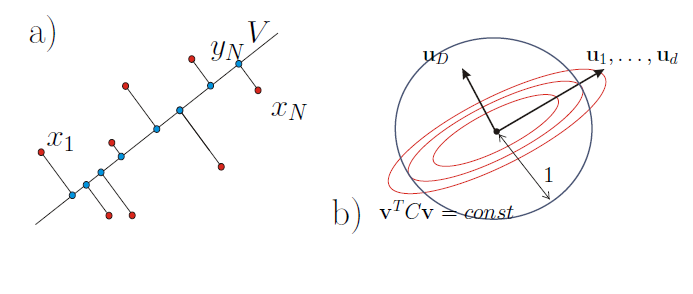
\includegraphics[width=\textwidth]{./Figures/pca.png}
\caption{a) Manifold with original (red) and projected (blue) points. b) Geometry and constraint visualization of optimization function. Pictures taken from Nicolas Thorstensen works \citep{Ety2008}}
\label{pca}
\end{center}
\end{figure}

Now, we can write the energy function as
\begin{equation}
\mathbb{E} = \frac{1}{N}\sum_{n=1}^{N}\sum_{i=d+1}^{D} (x_n^{T}u_{i}- \bar{x}^{T}u_i)^2 = \sum_{i=d+1}^{D}u_{i}^{T}\mathbf{C}u_{i}
\end{equation}

$\mathbf{C}$ is defined as covariance matrix, $\mathbf{C} = \frac{1}{N}\sum_{n=1}^{N}(x_n-\bar{x})(x_n -\bar{x})^2$. Our optimization problem look like
\begin{equation}
\begin{aligned}
& \underset{D}{\text{minimize}}
&& \mathbb{E} = u_{D}^{T}\mathbf{C}u_{D} \\
& \text{subject to}
&& u_{D}^{T}u_{D} = 1
\end{aligned}
\end{equation}
Now using Lagrange multipliers, we solve this constraint optimization problem as
\begin{equation}
u_{D}^{T}\mathbf{C}u_{D}+\lambda(1-u_{D}^{T}u_{D})=0
\label{LM}
\end{equation}

The solution off the above equation gives standard form eigenvalue problem $\mathbf{C}u_D =\lambda u_D$. The geometry of the minimization problem is illustrated in figure \ref{pca} b).

We take an input image \ref{app_pca} (A), which is sequence of vector in $\mathbb{R}^{4096}$ representing the brightness values of $64\times64$ pixel image of the face. The 1st dimension representing embedding correlates with intrinsic-dimension of one, which is left-right pose. The two-dimensional projection of original input image found by PCA is shown in figure \ref{app_pca} (B).

\begin{figure}
\centering
\begin{subfigure}{.5\textwidth}
  \centering
  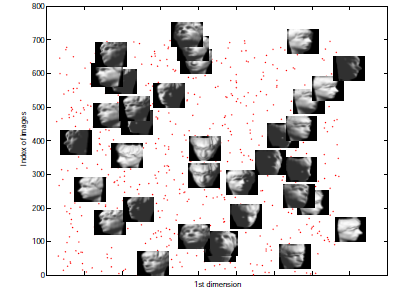
\includegraphics[width=\linewidth]{./Figures/original.png}
\caption{Input}
%  \label{fig:sub1}
\end{subfigure}%
\begin{subfigure}{.5\textwidth}
  \centering
  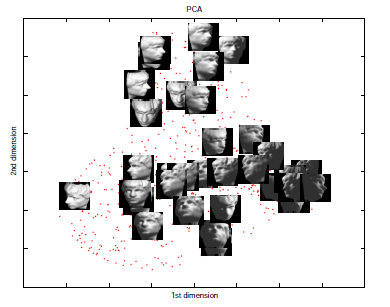
\includegraphics[width=\linewidth]{./Figures/o_pca.png}
  \caption{Output}
%  \label{fig:sub2}
\end{subfigure}
\caption{Application of PCA. }
\label{app_pca}
\end{figure}

\subsection{Multi-Dimensional Scaling}
\label{s:MDS}

The Multi-Dimensional Scaling (MDS), is a PCA-like technique that maps the original high dimensional space to a lower dimensional space by preserving pairwise distances. Figure \ref{app_mds} shows an example of MDS, where pairwise distance is preserved. MDS \citep{Cox2000} is applied when it difficult to calculate   covariance matrix from the dataset, when data are, for instance, qualitative or infinite dimensional, when only a point-wise distance is known or also when the size $\mathbb{D}$ of the sample set is lower than the dimension of data \citep{Ety2008}.


MDS addresses the problem of finding d-dimensional Euclidean coordinates
for each data sample ($x_i \in \mathbf{X}$) so that the pairwise distance ($d$) of their Euclidean coordinates match the original pairwise distance as closely as possible. 

We define $N \times N$ euclidean distance or affinity matrices $\mathbf{D}$ as symmetric, $d_{ii}=0$ and $d_{ij}>0$, if $i \neq j$. With $\mathbf{D}$ matrix in hand, the MDS algorithm attempts to find $N$ data points $\mathbf{Y} = y_1, y_2, y_3,...,y_N$ in $\mathbb{R}^d$ such that distance matrix is preserved as depicted in the figure \ref{mds}.


\begin{figure}
\centering
\begin{subfigure}{.5\textwidth}
  \centering
  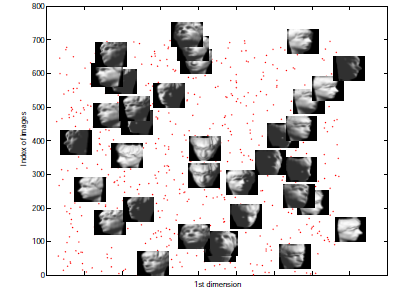
\includegraphics[width=\linewidth]{./Figures/original.png}
\caption{Input}
%  \label{fig:sub1}
\end{subfigure}%
\begin{subfigure}{.5\textwidth}
  \centering
  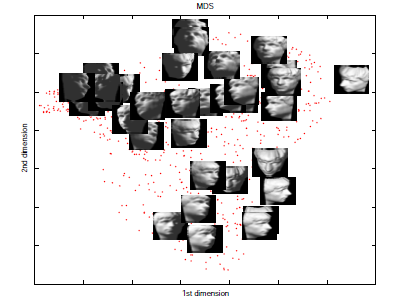
\includegraphics[width=\linewidth]{./Figures/o_mds.png}
  \caption{Output}
%  \label{fig:sub2}
\end{subfigure}
\caption{Application of MDS.}
\label{app_mds}
\end{figure}

\begin{figure}[ht]
\begin{center}
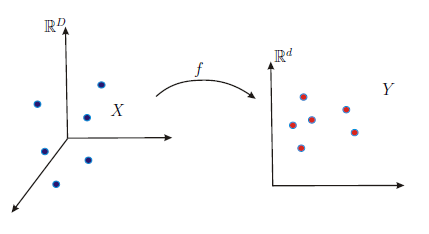
\includegraphics[width=\textwidth]{./Figures/mds.png}
\caption {Multi-Dimensional Scaling}
\label{mds}
\end{center}
\end{figure}

In particular, we try to optimize following function:

\begin{equation}
\begin{aligned}
& \underset{\mathbf{Y}}{\text{Min}}
&& \sum_{i=1}^{N}\sum_{i=1}^{N}(d_{ij}^{\mathbf{X}}-d_{ij}^{\mathbf{Y}})^{2}
\label{mds:1}
\end{aligned}
\end{equation}

where, $d_{ij}^{\mathbf{X}}$ and $d_{ij}^{\mathbf{Y}}$ is normed distance from sample point $x_{i}$ and $x_{i}$ respectively. Converting distance $\mathbf{D}^{\mathbb{X}}$ matrix into kernel matrix of inner product yields:

\begin{equation}
\mathbf{X}^{T}\mathbf{X} = -\frac{1}{2}\mathbf{J}\mathbf{D}^{\mathbb{X}}
\end{equation}
where $\mathbf{J} = \mathcal{I}d_{N}-\frac{1}{N}\mathbf{1}\mathbf{1}^{T}$. Now the equation \ref{mds:1} can be reduced into

\begin{equation}
\begin{aligned}
& \underset{\mathbf{Y}}{\text{Min}}
&& \sum_{i=1}^{N}\sum_{i=1}^{N}(x_{i}^{T}x_{j}-y_{i}^{T}y_{j})^{2}
\label{mds:2}
\end{aligned}
\end{equation}


Solving equation \ref{mds:2} as shown in Cox and Cox paper\citep{Cox2000} gives $\mathbf{Y}=\lambda^{\frac{1}{2}}\mathbf{U}^{T}$. Here, $\mathbf{U}$ is eigenvector of $\mathbf{X}^{T}\mathbf{X}$ corresponding to top d eigenvalues, and $\lambda$ is top d eigenvalues of $\mathbf{X}^{T}\mathbf{X}$.


MDS can be generalized into to geodesic distances between point samples from
a non-linear manifold. But a non-convex energy function coming out makes it  
tedious to optimize. In the next section we will provide an overview of non-linear manifold algorithms.


\section{Non-Linear Methods}

Linear methods such as PCA and MDS fails to produce desired results when the data is sampled from non linear manifolds \citep{Thor2009}. We now review representative non-linear methods in manifold learning in this section with assumption that the data is distributed along a d-dimensional submanifold $\mathcal{X}$ embedded in $\mathbb{R}^{D}$.

\subsection{Graph-based Algorithms}

Manifold learning based on graph based algorithms often relies on preserving the geometric structure in the neighborhood of some points. The important step is to construct a graph using $K$-nearest neighbor graph or $\epsilon$-neighborhood and apply MDS as previously detailed.

\subsubsection{Isomap}
\label{s:isomap}

Isomap was proposed by Joshua Tenenbaum, Vin de Silva and John Langford in Science \citep{Tene2000}. It is an extended version of MDS for data lying on smooth non-linear manifold. Unlike MDS, the pairwise distance matrix in Isomap is replaced by the matrix of pairwise geodesic distances approximated by distances in graphs. The algorithm proceeds in three steps. First a distance $d(x; y)$ is considered in the data space. Then, a neighborhood graph based on a $\epsilon$-neighborhood or $k$-nearest neighbor points is build with following weights $D_{ij} = d(xi; xj)$ if an edge link
exists between points $x_i$ and $x_j$ , otherwise $D_{ij} = 1$. The pairwise distance matrix $\mathbf{D}$ is then calculated using a Dijkstra-like algorithm in the graph. Finally, the data via MDS is embedded so as to preserve these distances. A two-dimensional projection using isomap is shown in the figure \ref{app_iso} with k=6.

\begin{figure}
\centering
\begin{subfigure}{.5\textwidth}
  \centering
  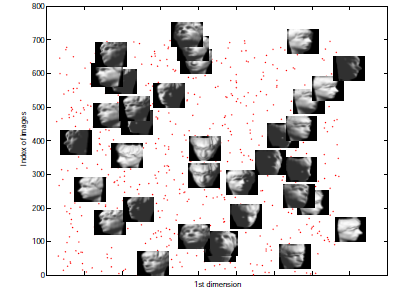
\includegraphics[width=\linewidth]{./Figures/original.png}
\caption{Input}
%  \label{fig:sub1}
\end{subfigure}%
\begin{subfigure}{.5\textwidth}
  \centering
  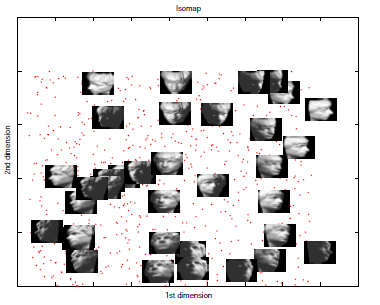
\includegraphics[width=\linewidth]{./Figures/o_iso.png}
  \caption{Output}
%  \label{fig:sub2}
\end{subfigure}
\caption{Application of Isomap}
\label{app_iso}
\end{figure}

Precautionary measure should be taken while calculating distances between far apart points on the manifold, which can be very close in the data space as discussed in the figure \ref{isomap}.
\begin{figure}[ht]
\begin{center}
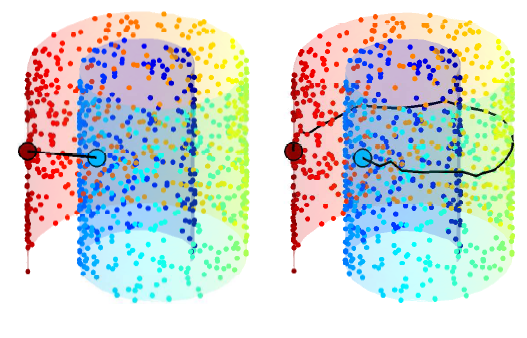
\includegraphics[width=\textwidth]{./Figures/isomap.png}
\caption {Multi-Dimensional Scaling. Left: Distance between two
points using a distance in the data space. Right: Distance between two points
using an approximated geodesic path. Image taken from Patrick Etyngier work \citep{Ety2008}.}
\label{isomap}
\end{center}
\end{figure}

\subsubsection{Locally linear Embedding}
\label{s:lle}
Locally linear Embedding (LLE) is a manifold mapping dimension reduction algorithm introduced by Roweis \& Saul \citep{Roweis2000}. It aims at recovering the low dimensional geometry of the data by looking at the local interaction between data points. The construction of a nearest neighbor graph recovers the local interactions. Then further processing is done to reduce the dimensionality of the data and provide a parametrization in a d- dimensional hyperplane. LLE algorithm can be summarized in the following steps:

\begin{enumerate}
\item  Neighborhood graph $\mathcal{G}$ is build on the dataset $\mathbb{X}$ using K-nearest neighbour method. 
\item Weights $W_{ij}$ are calculated to each of the nearest neighbours pair $(x_i, y_i)$ by minimising the cost function:
      \begin{equation}
     \epsilon(W) = \sum_{i}\vert x_{i} - \sum_{j=1}^k W_{ij} x_{j}\vert^{2}
    \end{equation}
   
\item The inner products between each point $x_i$ and each of its nearest neighbours are computed to produce gram positive-semidefinite matrix, $G_{jk} = (x -x_j)^T(x-x_i)$.
\item  The reconstruction weights are then computed using:
    \begin{equation}
     W_{ij} = \sum_{k}\mathbb{G}-{jk}^{-1}(G_{jk}+\lambda)
    \end{equation}
    such that, $W_{ij} =0 $ if $x_{j}$ is not one of the nearest neighbours of $x_{i}$ and $\sum_{j} W_{ij} = 1$)
    
\item Finally the embedded $\mathbb{Y}$ which will make up the final output data are calculated by minimising a second cost function:
    \begin{equation}
     \Phi(Y) = \sum_{i}\vert y_{i}-\sum_{j}W_{ij}y_{j}\vert^{2}
    \end{equation}
We also constraint $\sum_{i}y_{i} = 0$ to centre the projection on the origin. The other constraint is imposed in order to avoid degenerate solutions;
    \begin{equation}
     \frac{1}{n}\sum_{i}y_{i}y_{i}^{T} = I
    \end{equation}
    where I is the d$\times$d identity matrix.
    
\item     This cost function now defines a quadratic form containing the N$\times$N symmetric matrix $M_{ij}$:
    \begin{equation}
     \Phi(I) =\sum_{ij}M_{ij}y_{i}y_{i}^{T}
    \end{equation}
    where $M_{ij} = \delta_{ij}-W_{ij}-W_{ij}+\sum_{k}W_{ki}W_{kj}$ and $\delta_{ij} = 1$ if $i = j$ and $\delta_{ij} = 0$ otherwise.
\item The embedding $\mathbb{Y}$ is then given by the the lowest d+1 eigenvectors of the matrix $M_{ij}$. The bottom eigenvector representing a 
free translation mode of eigenvalue 0 is left out in order to find the optimum embedding.

\end{enumerate}

The geometry the optimization problem is depicted in figure \ref{lle}.

\begin{figure}[ht]
\begin{center}
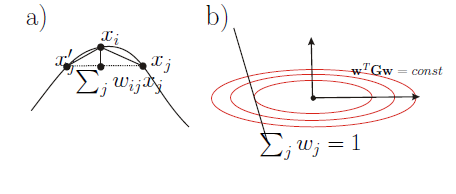
\includegraphics[width=\textwidth]{./Figures/lle.png}
\caption {LLE. a) $x_i$ is appropriated by its neighborhood $(x_{j}^{'}, x_{j})$. b) The black line touching the level set at a single point defines the constraints}
\label{lle} 
\end{center}
\end{figure}

A two-dimensional projection of the original input by using with k=5 is shown in the figure \ref{app_lle}.
\begin{figure}
\centering
\begin{subfigure}{.5\textwidth}
  \centering
  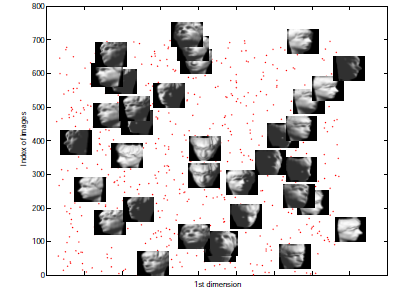
\includegraphics[width=\linewidth]{./Figures/original.png}
\caption{Input}
%  \label{fig:sub1}
\end{subfigure}%
\begin{subfigure}{.5\textwidth}
  \centering
  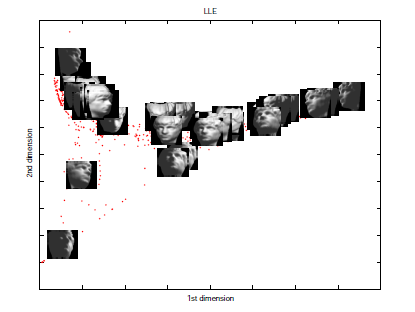
\includegraphics[width=\linewidth]{./Figures/o_lle.png}
  \caption{Output}
%  \label{fig:sub2}
\end{subfigure}
\caption{Application of LLE}
\label{app_lle}
\end{figure}

\subsection{Laplacian-based Algorithms}
Laplacian based algorithms assume that data have a structure of low dimensional manifold embedded in a higher dimensional space. The maps are constructed into a low dimensional space preserving the local neighborhood topology. In this part, we give outlines of representative laplacian based algorithms.

\subsubsection{Laplacian Eigenmaps}
\label{s:le}
Laplacian Eigenmaps were introduced by Belkin \citep{Bel2002}. Its intent is
to embed the observed data $\mathbf{X}$ into $\mathbb{R}^d$ by first constructing the $k$-nearest-neighbor or $\epsilon$-graph $\mathcal{G}$ from $\mathbf{X}$. In the $k$-nearest-neighbor graph, an edge is present between $x_i$ and $x_j$ if $x_i$ is among the $k$ nearest neighbors of $x_j$ or vice versa. In the $\epsilon$-graph, $x_i$ and $x_j$ are adjacent if $\|x_i-x_j\|^2<\epsilon$ for a given threshold parameter $\epsilon$. The weighted adjacency matrix of $\mathcal{G}$ is defined as $\mathbf{W}$, $$\mathbf{W}_{ij}=\begin{cases} \mathbf{K}_{ij} &\mbox{ if } \{i,j\}\in E\\
                0 &\mbox{ else}, \end{cases}$$ and let $\mathbf{D}\in\mathbb{R}^{N\times N}$ be the diagonal matrix defined by $\mathbf{D}_{ii}=\sum_{j}\mathbf{W}_{ij}$ for $i\in[N]$.
                
Then the normalized weighted graph Laplacian of $\mathbf{G}$ \citep{Bel2002}
is given by $\mathbf{W}=\mathbf{D}^{-1/2}\mathbf{W}\mathbf{D}^{-1/2}$.
If we represent eigendecomposition of $\mathbf{W}$  by $\mathbf{W}=\mathbf{U}\Lambda \mathbf{U}^\top$ with the diagonal entries of $\Lambda$ non-increasing, then Laplacian eigenmaps embeds $\mathbf{X}$ via
$\mathbf{U}[:,2:d+1]$---the first $d$ nontrivial eigenvectors of $\mathbf{W}$. The local geometry of $\mathbf{X}$ is optimally preserved in a least squares sense by the former.
 
A two-dimensional projection of the original input by using with k=9 is shown in the figure \ref{app_le}.
 
\begin{figure}
\centering
\begin{subfigure}{.5\textwidth}
  \centering
  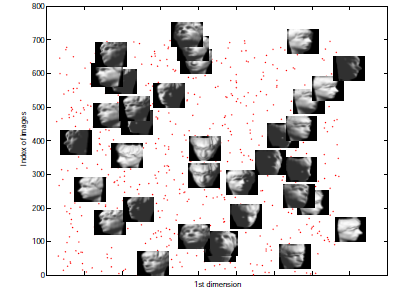
\includegraphics[width=\linewidth]{./Figures/original.png}
\caption{Input}
%  \label{fig:sub1}
\end{subfigure}%
\begin{subfigure}{.5\textwidth}
  \centering
  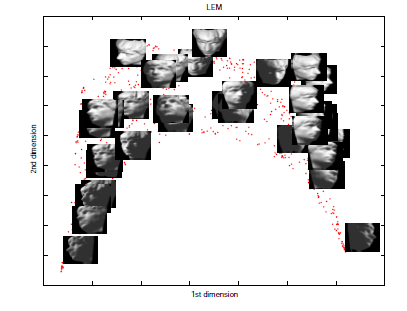
\includegraphics[width=\linewidth]{./Figures/o_le.png}
  \caption{Output}
%  \label{fig:sub2}
\end{subfigure}
\caption{Application of Laplacian Eigenmaps}
\label{app_le}
\end{figure}



\subsubsection{Diffusion Maps}
\label{s:dm}

The objective of Diffusion Maps (DM) is to define a metric, named the diffusion distance, that measures the connectivity between points in an arbitrary set. We will follow the construction of DM as described
in the paper by Lindenbaum and others \citep{Lind2015}.

Representing the high dimensional input dataset \begin{math} \mymat{X} \end{math}, the DM framework contains the following steps:

\begin{enumerate}

\item A kernel function  \begin{math}{{\cal{K}} : \mymat{X}\times{\mymat{X}}\longrightarrow{\mathbb{R}}  }
	\end{math} is chosen to define an anisotropic transition matrix, represented by $\mymat{K} \in {\mathbb{R}^{D \times D}}$. It satisfies the following properties for all 
	\begin{math}{(\myvec{x}_i,\myvec{x}_j) \in {\mymat{X}} }
	\end{math}.
	
	\begin{enumerate}
	
     \item Symmetry: \begin{math}{K_{i,j}={\cal{K}}(\myvec{x}_i,\myvec{x}_j)={\cal{K}}(\myvec{x}_j,\myvec{x}_i) }
	\end{math}, 
	
	\item Positive semi-definiteness: \begin{math}{ \myvec{v}_i^T  \mymat{K}  \myvec{v}_i \geq 0 }\end{math} for all $\myvec{v}_i \in
	\mathbb{R}^D$ and 
	
	\item Non-Negativity \begin{math}{{\cal{K}}(\myvec{x}_i,\myvec{x}_j)
		\geq 0. }
	\end{math}
	\end{enumerate}
	
\item {When we normalize the kernel using  $\mymat{M}$; where  \begin{math} M_{i,i}=\underset{j}{\sum}{K_{i,j}} \end{math}, the following matrix elements are computed:  
\begin{equation}
		{P_{i,j}^x={\cal{P}}(\myvec{x}_i,\myvec{x}_j)=[{{\mymat{M}}^{-1}{\mymat{K}}  }}]_{i,j}
		\label{EquationPDM}
		.\end{equation}
		
		 The resulting matrix $ \mymat{P}^x \in \mathbb{R}^{D
			\times D} $ is actually transition kernel of a 
		Markov chain on $\mymat{X}$ such that the expression
		${[{(\mymat{P}^x)^t}]_{i,j}}=p_t(\myvec{x}_i$,$\myvec{x}_j)$
		describes the transition probability from point
		\begin{math}{\myvec{x}_i}
		\end{math} to point \begin{math}{\myvec{x}_j}
		\end{math} in $t$ steps.
	}
\item{ Next, the spectral decomposition is applied to matrix \begin{math}  \mymat{P}^x \end{math} to obtain a sequence of eigenvalues  \begin{math}{\lbrace {\lambda_d}\rbrace }
		\end{math} and normalized eigenvectors \begin{math}{\lbrace{{\mbox{\boldmath${\psi}$}}_d}\rbrace }
		\end{math} that satisfies ${ {\mymat{P}^x}  {\mbox{\boldmath${\psi}$}_d} =\lambda_m{\mbox{\boldmath${\psi}$}}_d, d=0,...,D-1}
		$; }
\item{
		Defining a new representation for the dataset $\mymat{X}$
		\begin{equation}{ \myvec{\Psi}_t{(\myvec{x}_i)}:   \myvec{x}_i
			\longmapsto \begin{bmatrix} { \lambda_1^{t}\psi_1[i]} , {
				\lambda_2^{t}\psi_2[i]} , { \lambda_3^{t}\psi_3[i]} , {.} {.} {.}
			,
			
			{\lambda_{D-1}^{t}\psi_{D-1}[i]}\\
			
			\end{bmatrix}^T \in{\mathbb{R}^{D-1}} },
		\end{equation}
		where $t$ is the selected number of steps and $\psi_d[i]$ denotes the $i^{\rm{th}}$ element of ${\mbox{\boldmath${\psi}$}_d}$.
		
Now the Euclidian distance between two data points is equal to the weighted $L_2$ distance between the conditional probabilities ${{p}_t(\myvec{x}_i,:)}$, and ${{p}_t(\myvec{x}_j,:)}$, $i,j=1,...,D$ (the $i$-th and $j$-th rows of $\myvec{P}^t$), which is referred as the Diffusion Distance
			\begin{equation}{ \label{EqDist} { {\cal{D}}^2_t( \myvec{x}_i,\myvec{x}_j)=||{\mymat{\Psi}_t{(\myvec{x}_i)}}-{\mymat{\Psi}_t{(\myvec{x}_j)}}||^2={  \sum_{d\geq{1}} {\lambda}^{2t}_d (\psi_d[i]-\psi_d[j])^2 }}=\\
			||{p_t}(\myvec{x}_i,:)-{p_t}(\myvec{x}_j,:)||^2_{\tiny\mymat{W}^{-1}}},
			\end{equation}
			where $\mymat{W}$ is a diagonal matrix with elements
			$W_{i,i}=\frac{D_{i,i}}{\sum_{i=1}^M D_{i,i}}$.}
	\item{The desired accuracy $\delta \geq 0$ is chosen for the diffusion distance defined by Eq. (\ref{EqDist}) such that
		$s(\delta,t)=\text{max} \{\ell\in \mathbb{N}$  such that   $|\lambda_{\ell}|^t > \delta |\lambda_1|^t \}  $. By using $\delta$, a new mapping
		of $s(\delta,t)$ dimensions is defined as \\ \begin{math} {\Psi^{(\delta)}_t :  X \rightarrow \begin{bmatrix}
			{ \lambda_1^{t}\psi_1[i]} , { \lambda_2^{t}\psi_2(i)} , {
				\lambda_3^{t}\psi_3[i]} , {.} {.} {.}   ,
			
			{\lambda_{s}^{t}\psi_{s}[i]}\\
			
			\end{bmatrix}^T \in \mathbb{R}^{s(\delta,t)}} \end{math} .  }
\end{enumerate}

As discussed above, diffusion distance reflects the intrinsic geometry of the data set defined via the adjacency graph in a diffusion process.

\section{Other manifold learning algorithms}

Many other Laplacian based techniques exist in literature to reduce the dimensionality of a point cloud which were not dicussed in this chapter. For example, Maximum Variance Unfolding (MVU)\citep{Ety2008}, which links most of Laplacian-based methods such as LE, LLE and Isomap. Another important approach which is derived from the LLE framework is called Hessian eigenmaps\citep{Ety2008}. The methods is widely used when the underlying embedding is not convex. In figure \ref{comp} taken from Thorstensen work \citep{Thor2009} lists the general properties for manifold learning algorithms.
%\begin{landscape}
\begin{figure}[ht]
\begin{center}
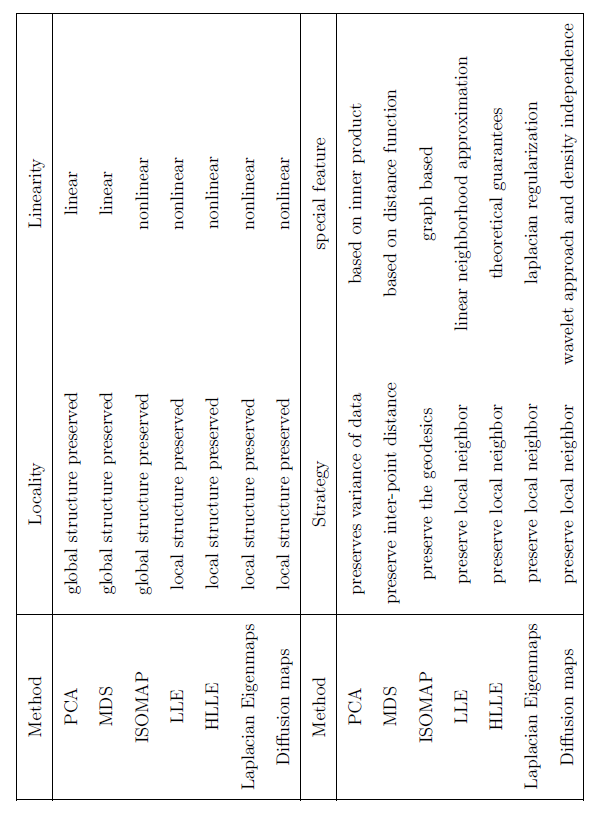
\includegraphics[width=\textwidth]{./Figures/comp_table.png}
\caption {Overview of Manifold Learning Algorithms}
\label{comp} 
\end{center}
\end{figure}
%\end{landscape}
\section{Intrinsic Dimension}
\label{s:id}

Intrinsic Dimension (ID) is defined as the minimal number of parameters necessary to represent the variability of a data set. It is a a key priori
knowledge in computer vision and image processing to improve their performance. Mathematically, a formal definition of the intrinsic dimension is the following, due to \citep{Cama2016}.

\begin{definition}
A data set $\mathbf{X}\subseteq \mathbb{R}^{\mathbf{D}}$ said to have intrinsic dimension equal to $\mathbf{d}$  if its elements lie entirely, without information loss, within a $\mathbf{d}$-dimensional manifold of $\mathbb{R}^{\mathbf{D}}$, where $\mathbf{d} < \mathbf{D}$.
\end{definition}

Most of the existing approach to estimate the intrinsic dimension can be roughly divided into two groups: eigenvalue or projection methods, and geometric methods. Projection or eigenvalues methods, estimate the ID by thresholding the observed eigenspectrum i.e. the spectrum of the eigenvalues output by the global or local PCA. It may be good method for exploratory
data analysis, where one might plot the eigenvalues and look for a clear-cut boundary, but not for providing reliable estimates of intrinsic dimension.

The other, geometric methods exploit the intrinsic geometry of the dataset and are most often based on fractal dimensions or nearest neighbor (NN) distances \citep{Lev2005}.

Finding out the ID of the dimension estimation might become a very complex problem, when data lie on a smooth manifold. In this thesis, we used method proposed by Levina and Bickel \citep{Lev2005} to verify the ID computed by projection and geometric methods. They derive ID by applying the principle of maximum likelihood to the distances between close neighbors. 
